\section{Passo 1 — Abrir a aplicação e criar o estudo}
\label{sec:passo1}

\subsection*{Objetivo}
Criar o \emph{estudo}, que guarda a configuração metodológica e todas as rodadas de busca de um mesmo
trabalho. O estudo é o contêiner; nada é calculado antes de existir uma rodada com arquivos.

\begin{figure}[H]
\centering
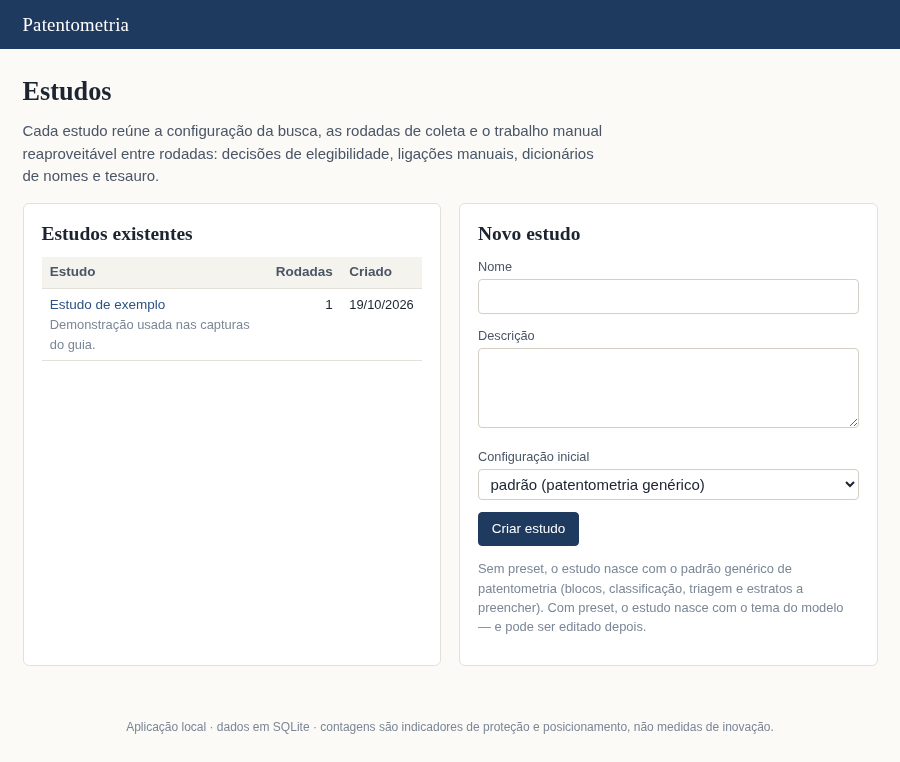
\includegraphics[width=0.95\linewidth]{img/01_home.png}
\caption{Tela inicial com a lista de estudos. No ambiente de demonstração existe um único estudo,
criado com o preset de exemplo.}
\label{fig:home}
\end{figure}

\subsection*{O que fazer}
\begin{enumerate}
\item Abra a aplicação (o instalador a inicia em \campo{http://127.0.0.1:8080}).
\item Confira se o estudo já existe na lista. Se existir, clique no nome.
\item Se não existir, preencha \textbf{Nome}, uma \textbf{Descrição} curta e escolha o preset
      \campo{vazio.json}.
\item Clique em \textbf{Criar estudo} e abra o estudo recém-criado.
\end{enumerate}

\subsection*{Como interpretar}
A lista mostra, para cada estudo, quantas rodadas ele tem. \textbf{Um estudo sem rodada é apenas um
formulário}: a configuração ainda não foi aplicada a nenhum corpus.

O nome deve identificar o recorte, não a instituição: ``Sensores ópticos em amostras ambientais'' é
melhor que ``Estudo 1''. A descrição é livre, mas vale registrar a pergunta que o estudo responde ---
ela será a chave para interpretar os indicadores depois.

\begin{nota}[Por que separar estudo e rodada]
A mesma pergunta pode ser respondida com buscas diferentes (bases diferentes, datas diferentes). Se
tudo ficasse em um único registro, não haveria como comparar duas coletas. A rodada é a foto datada;
o estudo é a regra do jogo.
\end{nota}

\begin{alerta}[Erro comum]
Criar um estudo novo para cada nova busca. Isso fragmenta o histórico. O correto é criar uma
\emph{rodada} dentro do mesmo estudo (Passo 3).
\end{alerta}

\subsection*{Checkpoint}
\marcador\; O estudo aparece na tela inicial e, ao abrir, mostra o painel com \textbf{0 rodadas}.
